\subsection*{a)}
Figure \ref{fig::4a} depicts the cross-section of an n-channel MOSFET at the onset of saturation. Note that a depletion region begins to exist near the drain as it acts like a reverse-biased diode with the substrate.
	\begin{figure}[htbp!]
	%	\centering
		\flushright
		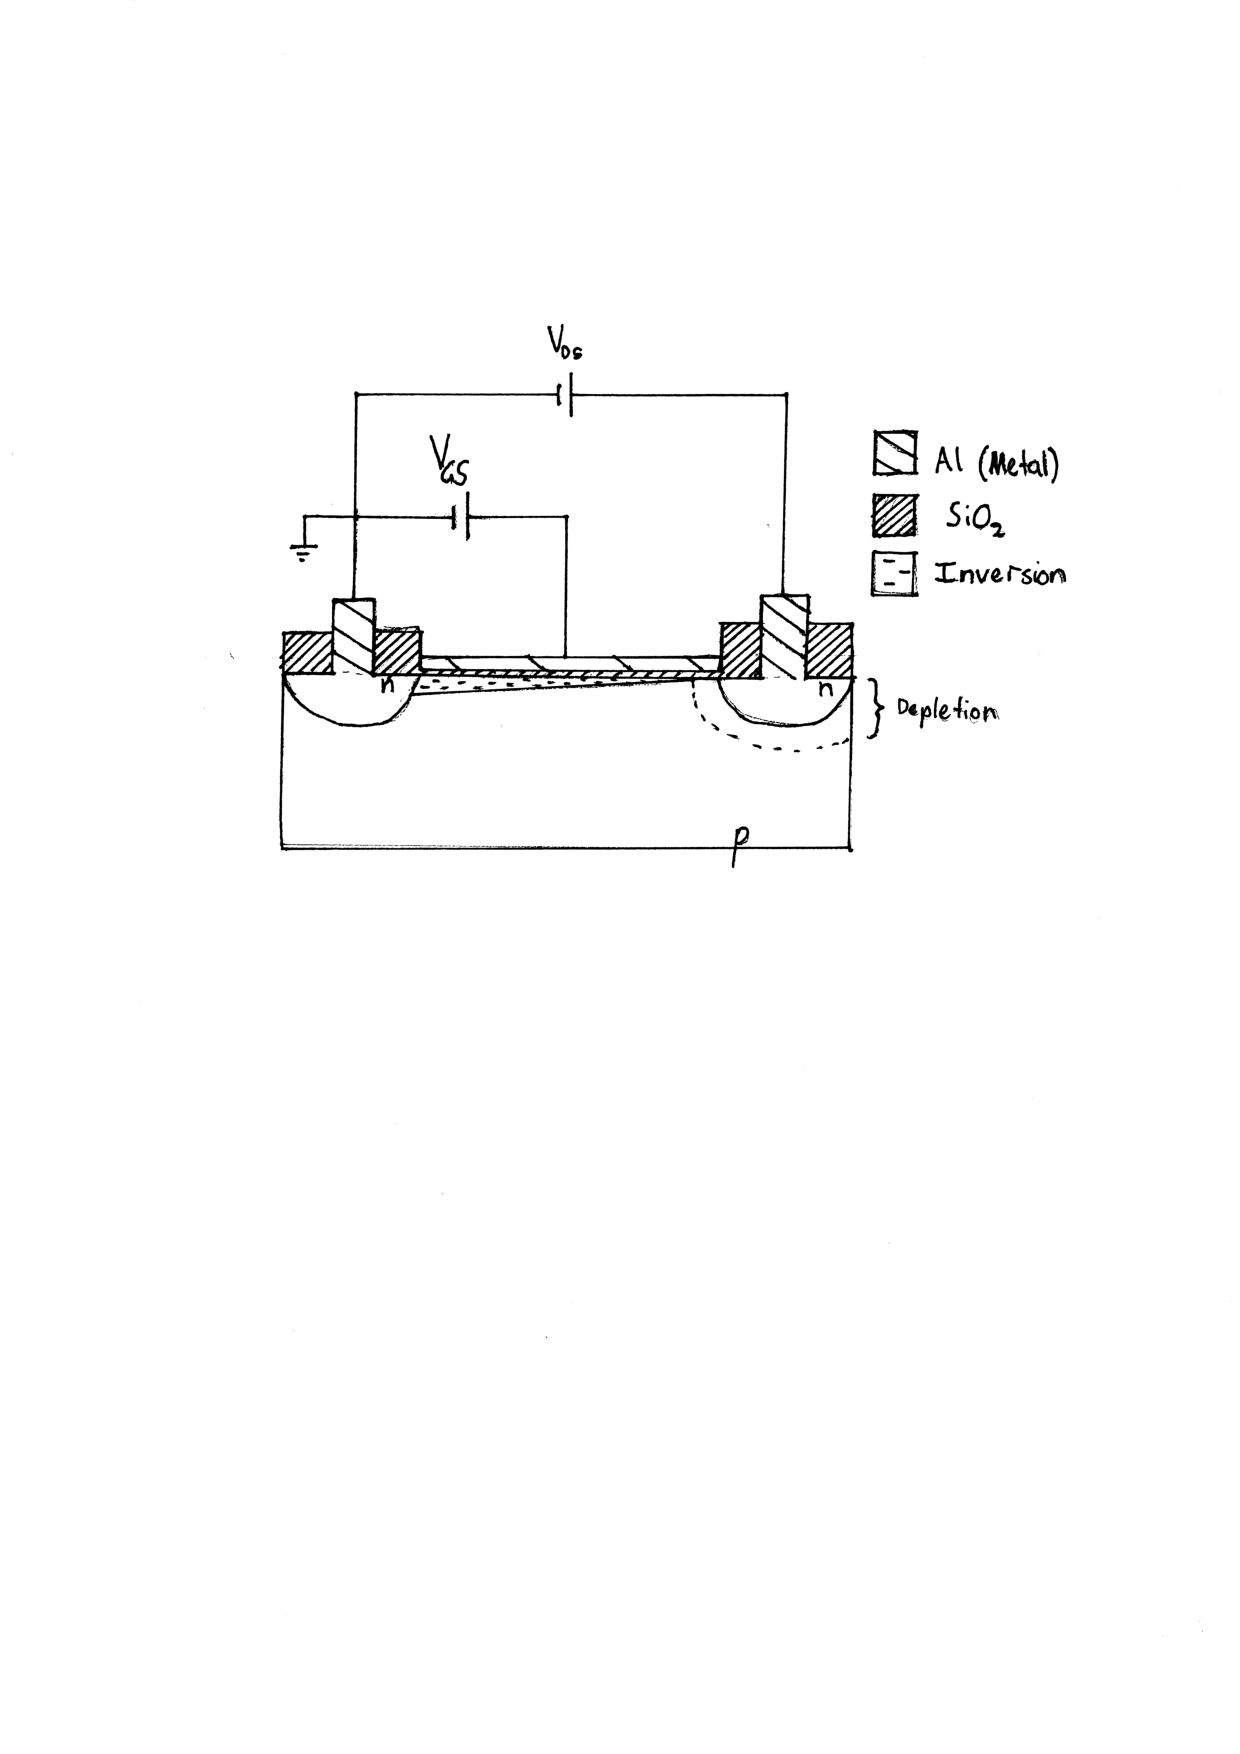
\includegraphics[trim={4cm 15cm 2.9cm 5cm},clip]{./img/4a}
		\caption{Cross-section of an n-channel MOSFET operating in saturation.}
		\label{fig::4a}
	\end{figure}
\subsection*{b)}
Assuming a flat-band between metal and semiconductor, the insulator is made from 1 nm thick silicon dioxide and an acceptor doping concentration of 
$N_A = 10^{19} \textrm{ cm}^{-3}$. Further, I will assume that the static interface charge, $Q_i$, is negligible.
\[
\begin{aligned}
	V_T &= 2 \phi_F - \frac{Q_s}{C_i} - \frac{Q_i}{C_i} \\
	V_T &= 2 \phi_F - \frac{Q_s}{C_i} \\
	\textrm{where}\\
	\phi_F	&= \frac{k T}{q} \ln \left(\frac{N_A}{n_i}\right) \\
		&= 25.9 \textrm{ mV} \cdot 20.7 \\
		&\approx 0.54 \textrm{ V} \\
	Q_s &= 2\sqrt{\epsilon_s q N_A \phi_F} \\
		&\approx 18.8 \textrm{ mC m}^{-2}\\
	C_i &= \frac{\epsilon_i}{d} \\
		&\approx 34.5 \textrm{ mF m}^{-2} \\
		%
		%
		\therefore V_T &= 2 \cdot 0.54 \textrm{ V} -
		 \dfrac{18.8  \textrm{ mC m}^{-2}}{34.5 \textrm{ mF m}^{-2}} \\
		 &= 0.53 \textrm{ V}
\end{aligned}
\]